\climbingarea{South Freeport Boulders}{%
    \climbheader{This is in Freeport..}{This is public access Land Trust land.}{Park at the Pine St/South Freeport Roard intersection pullout and walk back up Pine St 200 ft.}{The area is often wet, but The Coffin boulder stays dry.}

    \climbingarea{Grand Slab}{The first main area you get to from parking.}{%
        % A minipage is basically a small box of content that we will use to encapsulate our image. We will make it as wide as a line of text. This is used to maintain the formatting of the other text on the page.
        \begin{minipage}{\linewidth}%
          % We want to center the image within the minipage.
          \centering
          % This particular file is likely marked as "rotated" in the EXIF data, which LaTeX ignores...so we have to manually roate it here with the "angle" setting.
          % If you want the image smaller, you can change the width to '.5\linewidth' or some other value like that.
          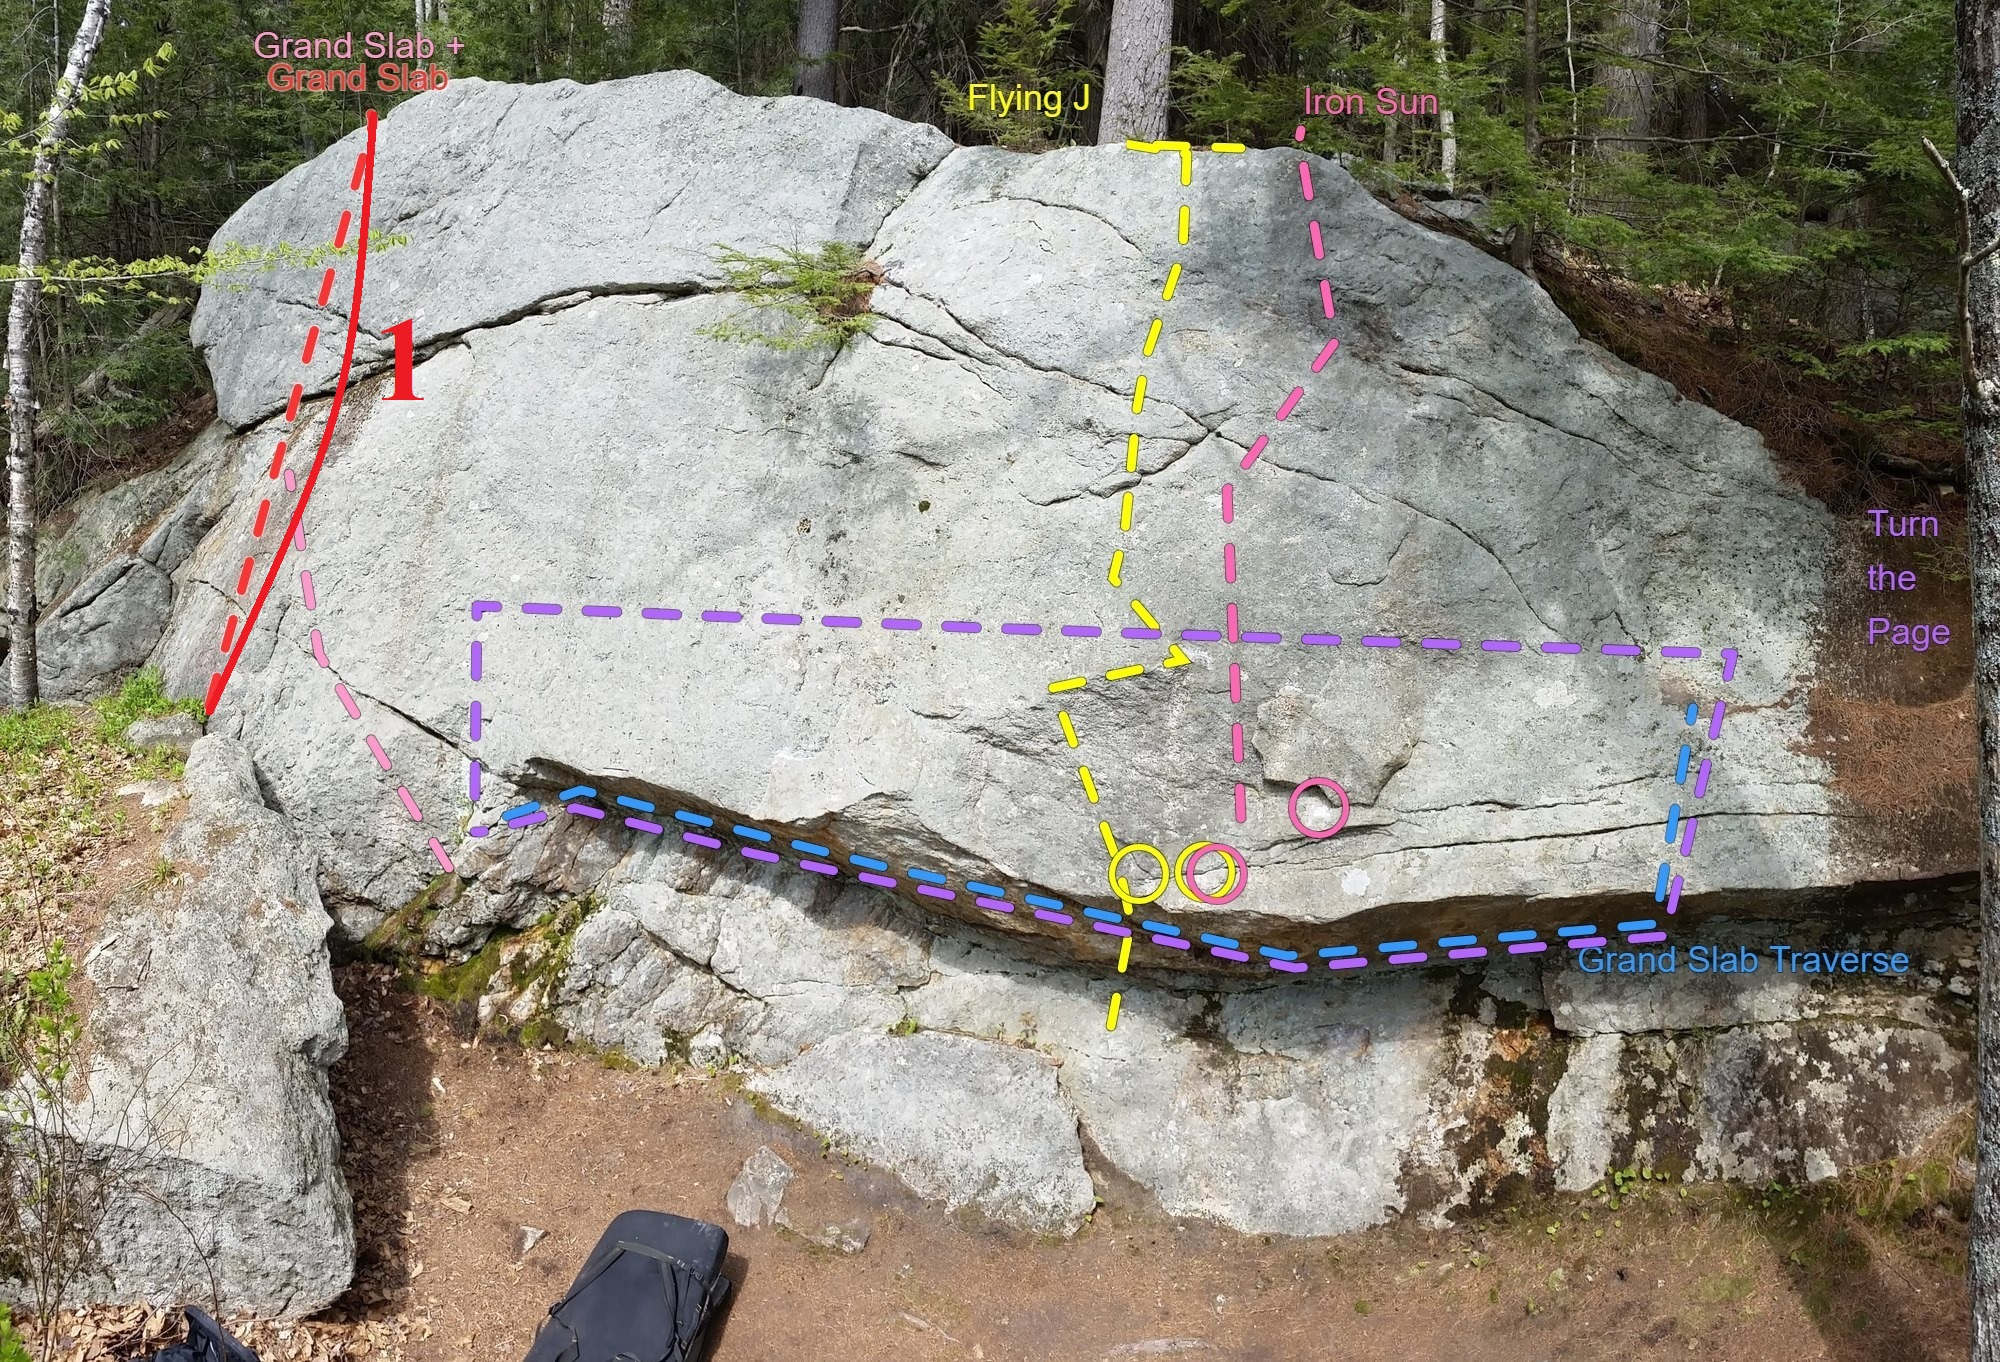
\includegraphics[angle=270,width=.8\linewidth]{GrandSlab.jpg}
          \captionof{figure}{Grand Slab boulder}
        \end{minipage}
        % This is a comment
        % the syntax of \boulderproblem is:
        % \boulderproblem[number of stars]{Name}{Grade}{Description}{Height}{FA}
        \boulderproblem[4]{Grand Slab}{V0}{From on top of the smaller boulder, stand-start and climb the left side of the slab using friction at the start and good edges at the end. Variation(V1): Start on the ground and climb up into the slab; the further right you stay, the harder.}{16}{unknown}
        \boulderproblem[4]{Grand Slab Traverse}{V1}{Stand-start one of the sides and traverse to the other. Drop off on the other end or top out via one of the other lines.}{10}{unknown}
        \boulderproblem[2]{Turn the Page}{V3/4}{Start anywhere and do a full circle of the low traverse into the high traverse (high roughly uses the hands of the low as feet). V3 clockwise, V4 counter-clockwise.}{40}{unknown}
        \boulderproblem[2]{Going Going/Gone}{V4}{Stand-start just to the left of the "in-the-way rock" on the good hands. Get feet high under the lip to reach the small crimp high left. Get foot just over the lip and do a big one leg squat to stand up on it. Work your way to the positive slab on the right (Going Going) or left (Gone) for the topout.}{18}{unknown}
        \boulderproblem[3]{Flying J}{V4}{Start on crimps just left of Iron Sun start. Either reach (tall beta) or do hand/foot coordination move (short beta) to get left hand on the slopy lip or get heel up on the shelf and then pull up to lip. Get right hand in the dish and then top out straight up. Top out left of the Iron Sun top half..}{17}{unknown}
        \boulderproblem[4]{Iron Sun}{V3}{Stand-start on crimps just above the lip and feet low. Get a high foot on the shelf to work your way up to the wide dishy pocket and then do several slab moves to topout.}{40}{unknown}
    }% Grand Slab
    
    \climbingarea{The Coffin Boulder}{The Coffin Boulder is pretty cool.}{%
        % A minipage is basically a small box of content that we will use to encapsulate our image. We will make it as wide as a line of text. This is used to maintain the formatting of the other text on the page.
        \begin{minipage}{\linewidth}%
          % We want to center the image within the minipage.
          \centering
          % This particular file is likely marked as "rotated" in the EXIF data, which LaTeX ignores...so we have to manually roate it here with the "angle" setting.
          % If you want the image smaller, you can change the width to '.5\linewidth' or some other value like that.
          \includegraphics[angle=270,width=.8\linewidth]{1201251115_HDR.jpg}
          \captionof{figure}{The Coffin V8/9}
        \end{minipage}
        % This is a comment
        % the syntax of \boulderproblem is:
        % \boulderproblem[number of stars]{Name}{Grade}{Description}{Height}{FA}
        \boulderproblem[4]{The Coffin}{V8/9}{Sit-start with hands on either arete with thumbcatch. Climb up the prow with compression, topping out to the left..}{10}{Ben Yunker?}
        \boulderproblem[4]{Podule}{V6}{Sit-start with hands on the right side of sloper cracks. Climb up and left on rough slopers.}{10}{unknown}
    }% Coffin Boulder
    
}{}% Freeport
